\chapter{Bayesian Statistics Implemented Through Markov Chain Monte Carlo Techniques}
\label{chap:MarkovChainMonteCarlo}
The analysis throughout this thesis is based upon a Bayesian oscillation analysis. To extract the oscillation parameters, a Markov Chain Monte Carlo (MCMC) method is used. This chapter explains the theory of how parameter estimates can be determined using this technique. \finish{Referenece MCMC Literature}.

The oscillation parameter determination presented within this thesis is built upon a simultaneous fit to near detector, far detector beam and atmospheric neutrino data. In total, there are four oscillation parameters of interest (\sinsqatm, \sinsqreac, \delmsqatm and \dcp), two oscillation parameters which this study will not be sensitive to (\sinsqsol, \delmsqsol) and  many nuisance parameters that control the systematic uncertainty models invoked within this study. The systematic uncertainties can be grouped into cateogries depending on how they are defined; \quickmath{574} bin-normalisations due to the near detector response, \quickmath{45} bin-normalisations to desccribe the far detector response to neutrino beam events, \quickmath{27} parameters to describe the detector response to atmospheric neutrino events, \quickmath{100} to model the bin-normalisation due to beam flux uncertanties, \quickmath{18} which model the atmospheric flux uncertainties, and \quickmath{87} to describe the correlated cross section model. An alternative parameterisation, where the far detector response is correlated between the beam and atmospheric samples, replaces the bin-normalisation parameters with \quickmath{224} shift and smear systematics. Section \finish{SystChap} describes the systematic model in more depth.

The MCMC technique generates a multi-dimensional probability distribution across all of the model parameters used in the fit. To determine the parameter estimate of a single parameter, this multi-dimensional object is integrated over all other parameters. This process is called Marginalisation and is further described in \autoref{sec:MarkovChainMonteCarlo_Marginalisation}. Monte Carlo techniques approximate the probability distribution of each parameter in the limit of generating many samples. As ever, generating a large number of samples is time and resource dependent and as such the MCMC technique is a clever algorithm which reduces the required number of samples to sufficiently sample the parameter space.

\section{Bayesian Statistics}
\label{sec:MarkovChainMonteCarlo_BayesianStatistics}
According to Bayesian Inference, observables and parameters of a statistical model are treated on an equal footing. To estimate model parameters \quickmath{\vec{\theta}} and data \quickmath{D}, one needs to define the joint probability distribution \quickmath{P(D|\vec{\theta}} which can be described as the prior distribution for model parameters \quickmath{P(\vec{\theta})} and the likelihood of the data given the model parameters \quickmath{P(D|\vec{\theta})},

\begin{equation}
  P(D,\vec{\theta}) = P(D|\vec{\theta})P(\vec{\theta}).
\end{equation}

The prior distribution, \quickmath{P(\vec{\theta})}, describes all previous knowledge about the parameters within the model. For example, if the risk of developing health problems is known to increase with age, the prior distribution would describe the increase. For the purpose of this analysis, the prior distribution are typically the best-fit values taken from external data measurements with a Gaussian unccertainty. The prior distribution can also contain correlations between model parameters. In an analysis using Monte Carlo techniques, the likelihood of measuring some data assuming some set of model parameters is calculated by comparing the Monte Carlo prediction generated at that particular set of model parameters to the data.

It is parameter estimation that is important for this analysis and as such, we apply Bayes' theorem \finish{Ref to Bayes' theorem} to calculate the probability for each parameter to have a certain value given the observed data \quickmath{P(\vec{\theta}|D)}, known as the posterior distribution (often just the posterior). This can be expressed as

\begin{equation}
  \label{eq:MarkovChainMonteCarlo_PosteriorDistribution}
  P(\vec{\theta}|D) = \frac{ P(D|\vec{\theta}) P(\vec{\theta}) }{ P(D|\vec{\theta}) P(\vec{\theta}) d\vec{\theta}}.
\end{equation}

The demoninator in \autoref{eq:MarkovChainMonteCarlo_PosteriorDistribution} is the integral of the joint probability distribution over all values of all parameters used within the fit. For brevity, we say that the posterior distribution is

\begin{equation}
  P(\vec{\theta}|D) \alpha P(D|\vec{\theta}) P(\vec{\theta}).
\end{equation}

In \autoref{sec:MarkovChainMonteCarlo_Marginalisation}, we see that for the cases used within this analysis, it is reasonable to know the posterior to some normalisation constant.

\section{Monte Carlo Simulation}
\label{sec:MarkovChainMonteCarlo_MonteCarloSimulation}
Monte Carlo techniques are used to numerically solve a complex problem. These techniques all rely on generating samples from a desired distribution and in the limit of high number of samples, approximate the properties of these samples as the properties of the distribution. A typical example of a simple use of Monte Carlo techniques is to calculate the area underneath a curve. For example, take the problem of calculating the area under a straight line with gradient \quickmath{M = 0.4} and constant \quickmath{C = 1.0}. Analytically, one can calculate the area under the line is equal to 3 units for \quickmath{0 \leq x \leq 10}. Using Monte Carlo techniques, one can calculate the area under this line by throwing many random values for the \quickmath{x} and \quickmath{y} components of each sample and then calculating whether that point falls below the line. The area can then be calculated by the ratio of points below the line to the total number of samples thrown multiplied by the total area of which samples were scattered. The study shown in \autoref{fig:MCMC_MCTechnique} highlights this technqiue and finds the area under the curve to be \quickmath{29.9} compared to an analytical solution of \quickmath{30.0}. The deviation of the numerical to analytical solution can be attributed to the number of samples used within the study. The accuracy of the approximation in which the properties of the Monte Carlo samples replicate those of the desired distribution is dependent on the number of samples used. Replicating this study with differing number of Monte Carlo samples used in each study (As shown in \autoref{fig:MCMC_MCTechniqueNThrowsStudy}) highlights how the Monte Carlo techniques are only accurate in the limit of high number of samples. Whilst this example has an analytical solution, these techniques are just as applicable to complex solutions. Clearly though, any numerical solution is only as useful as its efficiency. As discussed, the accuracy of the Monte Carlo technique is dependent upon the number of samples the problem is evaluated at. Furthermore if the positions at which the samples are evaluated are not cleverly picked, the efficiency of the Monte Carlo technique significantly drops. Given the example in \autoref{fig:MCMC_MCTechnique}, if the region in which the samples are scattered significantly extends passed the region of interest, many calculatations will be calculated but do not add to the ability of the Monte Carlo technique to achieve the correct result. For instance, any sample evaluated at a \quickmath{y \geq 5} could be removed without affecting the final result. This does bring in an aspect of the `chicken and egg' problem in that to achieve efficient sampling, one needs to know the distribution beforehand.

\begin{figure}[h]
  \begin{subfigure}[t]{0.80\textwidth}
    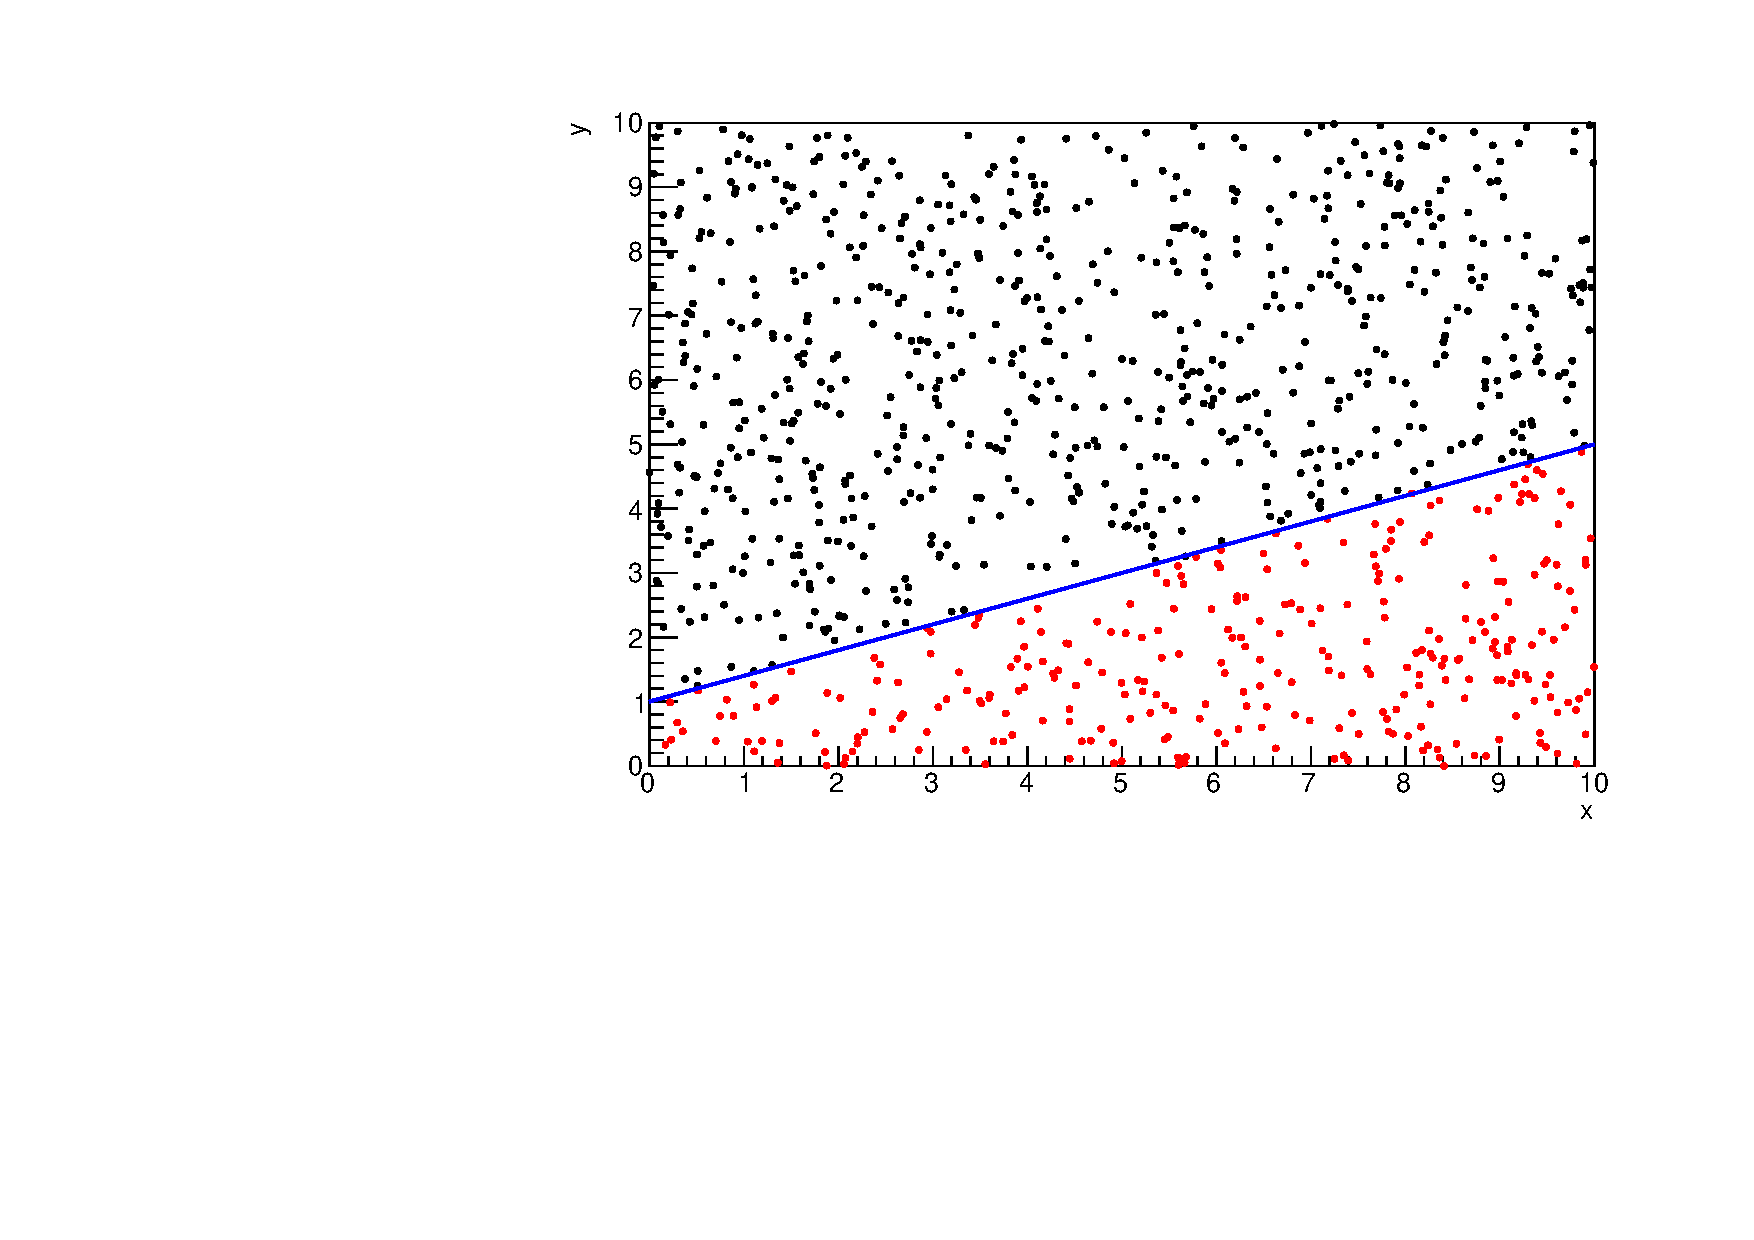
\includegraphics[width=\textwidth, trim={0mm 0mm 0mm 0mm}, clip,page=1]{Figures/MCMC/MCTechnique.pdf}
  \end{subfigure}
  \caption{Example of using Monte Carlo techniques to find the area under the blue line. The gradient and intercept of the line are \quickmath{0.4} and \quickmath{1.0} respectively. The area found to be under the curve using one thousand samples is \quickmath{29.9}.}
  \label{fig:MCMC_MCTechnique}
\end{figure}

\begin{figure}[h]
  \begin{subfigure}[t]{0.80\textwidth}
    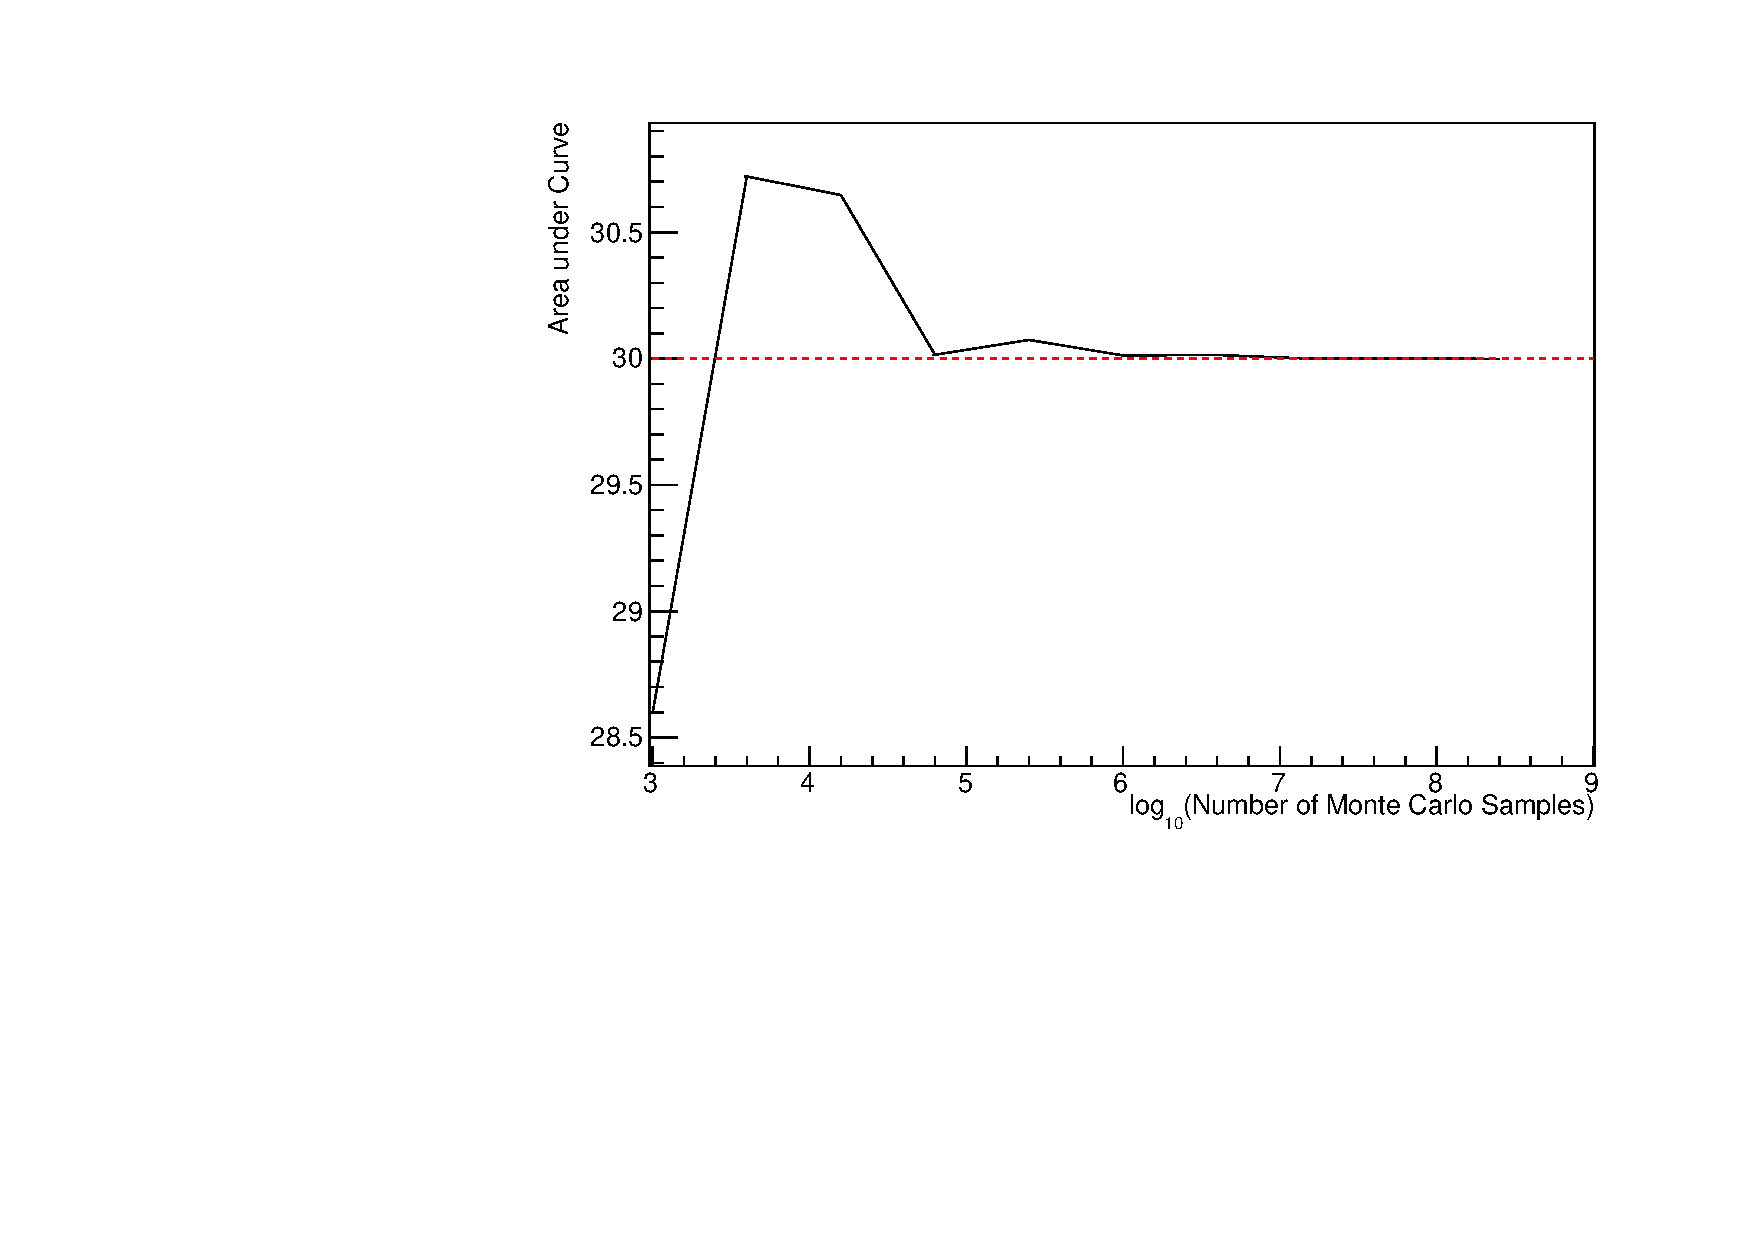
\includegraphics[width=\textwidth, trim={0mm 0mm 0mm 0mm}, clip,page=1]{Figures/MCMC/MCTechnique_NThrowsStudy.pdf}
  \end{subfigure}
  \caption{The area under a line of gradient \quickmath{0.4} and intercept \quickmath{1.0} for the range \quickmath{0 \leq x \leq 10} as calculated using Monte Carlo tecniques as a function of the number of samples used in each repetition. The analytical solution to the area is 30 units as given by the red line.}
  \label{fig:MCMC_MCTechniqueNThrowsStudy}
\end{figure}

\subsection{Markov Chain Monte Carlo}
\label{sec:MarkovChainMonteCarlo_MarkovChainMC}
This analysis utilises a multi-dimensional probability distribution, with some dimensions being significantly more constrained than others (whether that be from prior knowledge of parameter distributions from external data or un-physical regions in which parameters can not exist). Consequently, the Monte-Carlo techniques used need to be as efficient as possible. For this analysis, the Markov Chain Monte Carlo (MCMC) technique is choosen. An MCMC technique is a Monte Carlo technqiue which uses a Markov chain to select which points at which to sample tthe parameter distribution. This techniques performs a semi-random stochastic walk though the allowable parameter space, which builds the posterior distribution which has the property that the density of sampled points is proportional to the probability density of that parameter. This does mean that the samples produced by this technique are not statistically independent, but will cover the space of the distribution.

A Markov chain functions by selecting the position of step \quickmath{\vec{x}_{i+1}} based on the position of \quickmath{\vec{x}_{i}}. The space in which the Markov chain selects samples is dependent upon the total number of parameters utilised within the fit, where a discrete point in this space is descibed by the N-dimensional space \quickmath{\vec{x}}. In a perfectly operating Markov chain, the position of next step depends solely on the previous step and not on the further history of the chain (\quickmath{\vec{x}_{0}}, \quickmath{\vec{x}_{1}}, etc.). However, in solving the multi-dimesionality of the fit used within this analysis, each step becomes correlated with several of the steps procedding itself. This behaviour is further explained in \autoref{sec:MarkovChainMonteCarlo_MCMCOptimisation}. Providing the MCMC chain is well optimised, it will begin to converge towards a unique stationary distribution. The period between the chain's initial starting point and the convergence to the unique stationary distribution is colliqually known as burn-in period and is discussed further in \autoref{sec:MarkovChainMonteCarlo_MCMCOptimisation}. Once the chain reaches the stationary distribution, all points sampled after that pointt will looked like samples from that distribution.

Further details of the theories underpinning MCMC techniques are discussed in \finish{Link to MCMC techniques} but can be summarised by the requirement that the chain satifies the three `regularity conditions':

\begin{itemize}
\item Irreducibility: From every position in the parameter space \quickmath{\vec{x}}, there must exist a non-zero probability for every other position in the parameter space to be reached.
\item Recurrence: Once the chain arrives at the stationary distribution, every step following from that position must be samples from the same stationary distribution.
\item Aperiodicity: The chain must not repeat the same sequence of steps at any point throughtout the sampling period.
\end{itemize}

To then utilise MCMC techniques for parameter estimation, one needs to construct a Markov chain which has the property that the unique stationary distribution is the posterior distribution described in \autoref{sec:MarkovChainMonteCarlo_BayesianStatistics}. Consequently, the output of the chain after burn-in (ie. the sampled points after the chain has reached the stationary distribution) can then be used to approximate the posterior distribution and model parameters \quickmath{\vec{\theta}}. To achieve the requirement that the unique stationary distribution found by the chain be the posterior distribution, one can use the Metropolis Hastings algorithm which guides the stochastic process depending on the likelihood of the current proposed step compared to that of the previous step. Implementation and other details of this technique are discussed in \autoref{sec:MarkovChainMonteCarlo_MetropoliseHastingsAlgorithm}.

\subsection{Metropolis Hastings Algorithm}
\label{sec:MarkovChainMonteCarlo_MetropoliseHastingsAlgorithm}

As a requirement for MCMC, the Markov chain implemented in this technique must have a unique stationary distribution which is equivalent to the posterior distribution as highlighted in \autoref{sec:MarkovChainMonteCarlo_MetropoliseHastingsAlgorithm}. To ensure this requirement and that the regulairty conditions are met, this analysis utilises the Metropolis-Hastings algorithm \finish{M.H algorithm citations}. For the \quickmath{i^{th}} step in the chainn, this method determines the position in the allowable parameter space to which the chain steps to based on the current step, \quickmath{\vec{x}_{i}}, and the proposed step, \quickmath{\vec{y}_{i+1}}. The proposed step is randomomly selected from some proposal function \quickmath{f(\vec{x}_{i+1}|\vec{x}_{i})}, which depends solely on the current step (ie. not the further history of the chain). The next step in the chain \quickmath{\vec{x}_{i+1}} can be either the current step or the proposed step determined by whether the proposed step is accepted or rejected. To decide if the proposed step is selected, the acceptance probability, \quickmath{\alpha(\vec{x}_{i},\vec{y}_{i})}, is calculated as

\begin{equation}
  \label{eq:MarkovChainMonteCarlo_FullAcceptanceProbability}
  \alpha(\vec{x}_{i},\vec{y}_{i+1}) = min\left(1,\frac{P(\vec{y}_{i+1}|D)f(\vec{x}_{i}|\vec{y}_{i+1})}{P(\vec{x}_{i}|D)f(\vec{y}_{i+1}|\vec{x}_{i})} \right).
\end{equation}

Where \quickmath{P(\vec{y}_{i+1}|D)} is the posterior distribution as introduced in \autoref{sec:MarkovChainMonteCarlo_BayesianStatistics}. To simplify this calculation, the proposal function is required to be symmetric such that \quickmath{f(\vec{x}_{i}|\vec{y}_{i+1}) = f(\vec{y}_{i+1}|\vec{x}_{i})}. In practice, a multi-variate Gaussian distribution is used to throw parameter proposals from. This reduces \autoref{eq:MarkovChainMonteCarlo_FullAcceptanceProbability} to

\begin{equation}
  \label{eq:MarkovChainMonteCarlo_ReducedAcceptanceProbability}
  \alpha(\vec{x}_{i},\vec{y}_{i+1}) = min\left(1,\frac{P(\vec{y}_{i+1}|D)}{P(\vec{x}_{i}|D)} \right).
\end{equation}

After calculating this quantity, a random number, \quickmath{\beta}, is generated uniformally between 0 and 1. If \quickmath{\beta \leq \alpha(\vec{x}_{i},\vec{y}_{i+1})}, the proposed step is accepted. Otherwise, the chain sets the next step equal to the current step and this procedure is repeated. Consequently, one can notice that if the posterior probability of the proposed step is greater than that of the current step, (\quickmath{P(\vec{y}_{i+1}|D) \geq P(\vec{x}_{i}|D)}), the proposed step will always be accepted. If the opposite is true, (\quickmath{P(\vec{y}_{i+1}|D) \leq P(\vec{x}_{i}|D)}), the proposed step will be accepted with probability \quickmath{P(\vec{x}_{i}|D) / P(\vec{y}_{i+1}|D)}. This ensures that the Markov chain does not get trapped in any local minima present in the potentially non-Gaussian posterior distribution. The outcome of this technique is that the density of steps taken in a discrete region is directly proportional to the probability density in that region.

\subsection{MCMC Optimisation}
\label{sec:MarkovChainMonteCarlo_MCMCOptimisation}
As discussed in \autoref{sec:MarkovChainMonteCarlo_MetropoliseHastingsAlgorithm}, the proposal function invoked within the Metropolis Hastings algorithm can take any form and the chain will still converge to the stationary distribution; for this analysis a multi-variate Gaussian distribution was selected. As discussed in \finish{Link to Analysis Strategy}, this analysis performs the Monte Carlo reweighting on an event-by-event basis resulting in a large amount of computational resources required to perform a parameter fit. Consequently, the amount of steps taken before the unique stationary distribution is found should be minimised as only steps after convergence add information into the fit. Furthermore, the chain should entirely cover the allowable parameter space to ensure that all values have been considered. As a solution to both of these problems, tuning the distance that the proposal function jumps between steps on a parameter-by-parameter basis can both minimise the length of the burn-in period and ensure that the correlation between step \quickmath{\vec{x}_{i}} and \quickmath{\vec{x}_{i-n}}, where \quickmath{n} is some choosen number of steps away from the current step, is sufficientely small.

The effect of changing the width of the proposal function is highlighted in \autoref{fig:MCMC_MCTechniqueStepSizeStudy}. Three scenarios, each with the same underlying stationary distribution (A Gaussian of width \quickmath{1.0} and mean \quickmath{0.}), are presented. The only difference between the three scenarios is the width of the proposal function, colliqually known as the `step size', denoted \quickmath{f(\sigma)}, where \quickmath{\sigma} is the width of the Gaussian proposal function. Each scenario also starts at an initial parameter value of \quickmath{10.0} which would be considered an extreme variation, For the case where \quickmath{\sigma = 0.1}, it is clear to see that the chain takes a long time to reach the expected region of the parameter. This indicates that this chain would have a large burn-in period and would not converge to the stationary distribution until approximately step \quickmath{500}. Futhermore, whilst the chain does move towards the expected region, each step is signficantly correlated with the previous. Now considering the case where \quickmath{\sigma = 5.0}, the chain approachs the expected parameter region almost instantly meaning that the burnin period is not significant. However, there are clearly large regions of steps where the chain does not move as the chain proposes steps in the tails of the stationary distribution, with low probability of being accepted. Consequently, this chain would take a signficant number of steps to fully span the allowable parameter region. For the final scenario, where \quickmath{\sigma = 0.5}, you can see a relatively small burn-in period of approximately \quickmath{100} steps. Once the chain reaches the stationary distribution, it moves throughout the expected region of parameter values many times, sufficiently sampling the full parameter region. This example is a single parameter varying in across a continuous distribution and does not fully reflect the difficulties in the many-hundred multi-variate parameter distribution used within this analysis but it does give an conceptual idea of the importance of selecting the proposal function and associated step size. 

\begin{figure}[h]
  \begin{subfigure}[t]{\textwidth}
    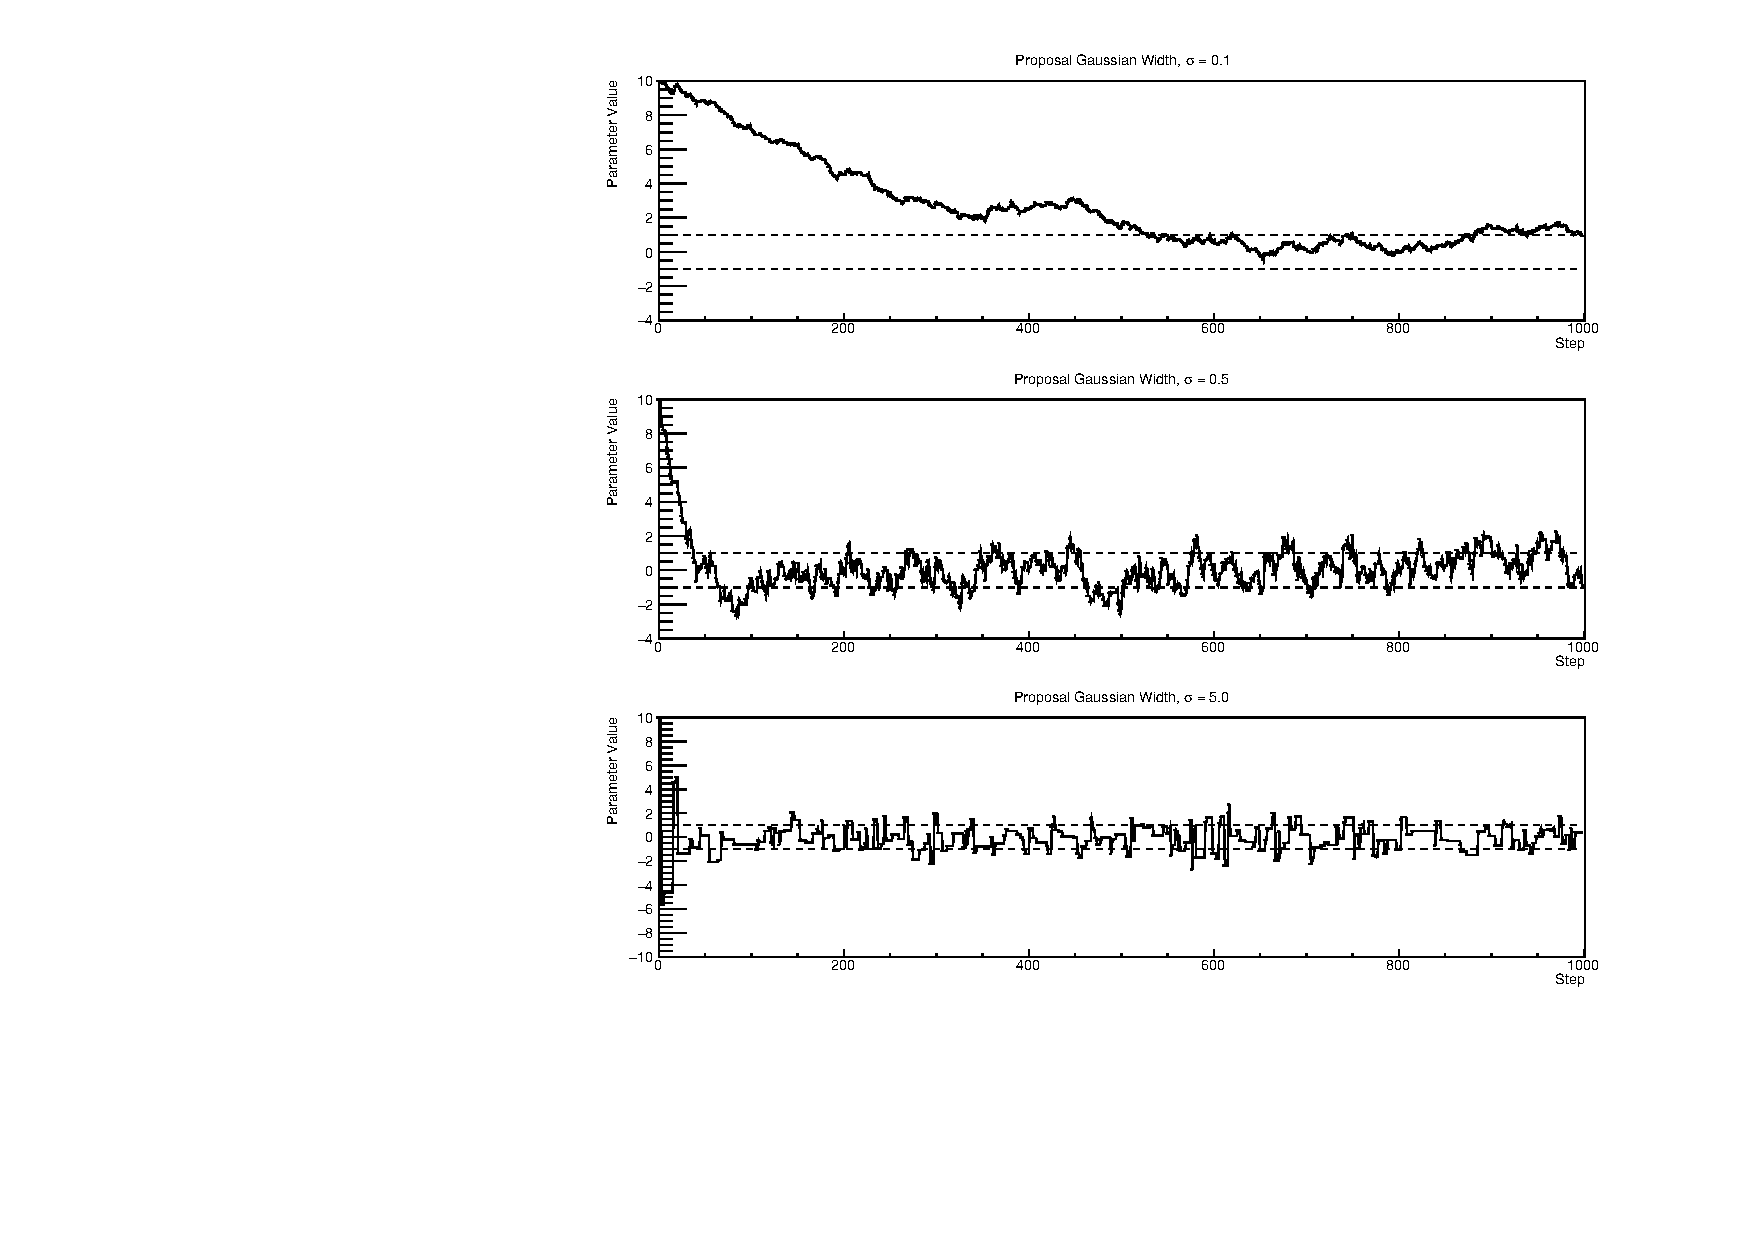
\includegraphics[width=\textwidth, trim={10mm 0mm 18mm 0mm}, clip,page=1]{Figures/MCMC/MCMCTechnique_StepSizes.pdf}
  \end{subfigure}
  \caption{Three MCMC chains, each with a stationary distribution equal to a Gaussian centered at \quickmath{0} and width \quickmath{1} (As indicated by the black dotted lines). All of the chains use a Gaussian proposal function but have different widths (or `step size \quickmath{\sigma}'). The top panel has \quickmath{\sigma = 0.1}, middle panel has \quickmath{\sigma = 0.5} and the bottom panel has \quickmath{\sigma = 5.0}.}
  \label{fig:MCMC_MCTechniqueStepSizeStudy}
\end{figure}

As discussed, step size tuning directly correlates to the number of steps the chain needs to have sufficient coverage of the full parameter space. It also directly ties into the average step acceptance rate. If the step size is too small, many steps will be accepted but the chain moves slowly. If the opposite is true, many steps will be rejected as the chain proposes steps in the tails of the distribution. Discussion in the literature \finish{Some juicy MCMC links} suggest that the `ideal' acceptance rate of a high dimension MCMC chain should be approximately \quickmath{\sim 25\%}. Many efforts have been taken to hand select a set of parameter-by-parameter step sizes to approximately reach the ideal acceptance rate.

\autoref{fig:MCMC_MCTechniqueStepSizeStudy} highlights the likelihood as calculated by the fit in \finish{Link to AsimovA official inputs section, also include in caption of \autoref{fig:MCMC_MCTechniqueStepSizeStudy}} as a function of the number of steps in each chain. In pratice, many independent MCMC chains are run simultaneously to parallelise the task of performing the fit. This figure overlays the distribution found from each chain. As seen, the likleihood decreases from it's initial value and converges towards a stationary distribution after \quickmath{1 \times 10^{5}} steps. As each fit (whether it be different asimov fits or data fit) will have a different set perfered parameter values which results in a different stationary distribution. For each fit in presented in this thesis, a burn-in period of \quickmath{1 \times 10^{5}} steps was found to be sufficient.

\begin{figure}[h]
  \begin{subfigure}[t]{\textwidth}
    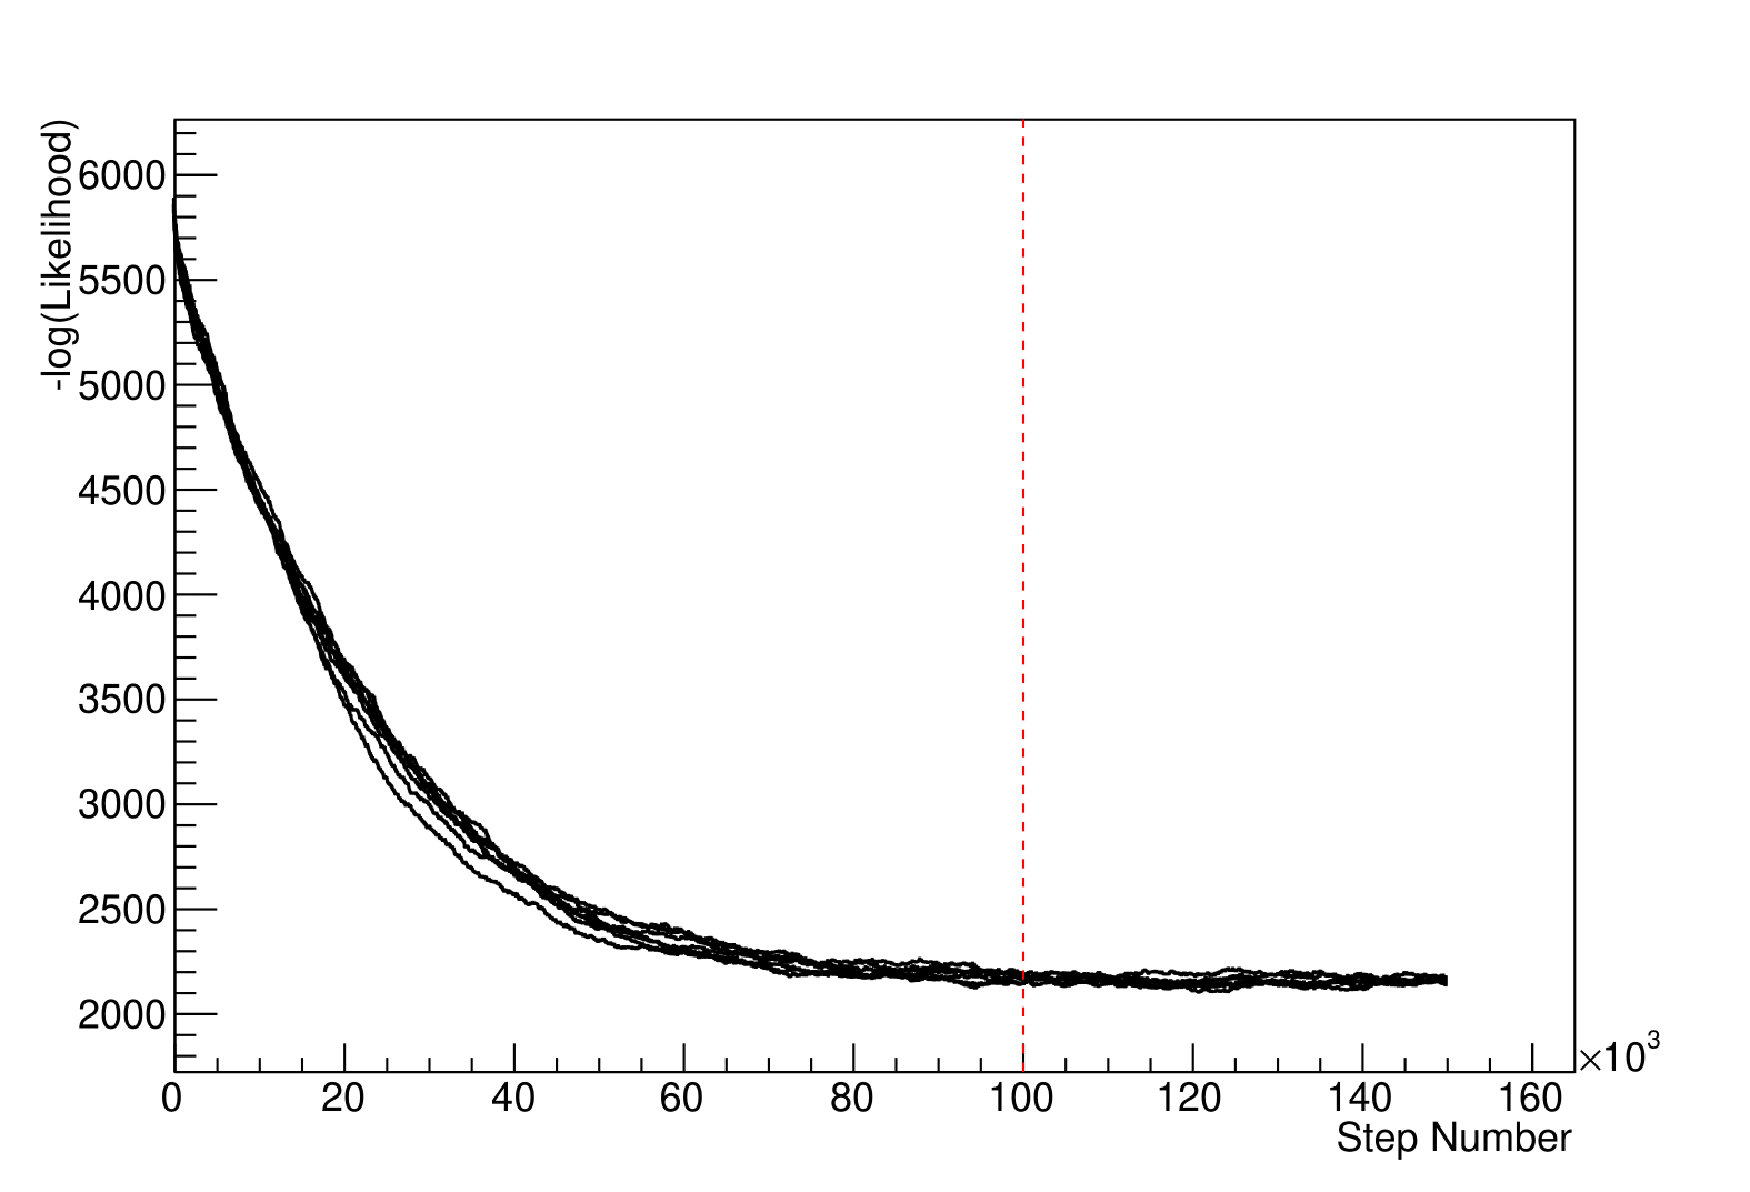
\includegraphics[width=\textwidth, trim={0mm 0mm 0mm 0mm}, clip,page=1]{Figures/MCMC/MCTechnique_LLHStep.pdf}
  \end{subfigure}
  \caption{The log-likelihood from the fit detailed in \finish{Link to AsimovA official inputs} as a function of the number of steps accumulated in each fit. Many independent MCMC chains were run in parallel and overlayed on this plot. The red line indicates the \quickmath{1 \times 10^{5}} step burn-in period after which the log-likelihood becomes stable.}
  \label{fig:MCMC_MCTechniqueLLHVsStep}
\end{figure}

\section{Parameter Estimation}
\label{sec:MarkovChainMonteCarlo_ParameterEstimation}

\subsection{Maginalisation}
\label{sec:MarkovChainMonteCarlo_Marginalisation}
